% abthmsnp.tex
% Application-based TCP Hijacking
% Author: Oliver Zheng / Jason Poon / Konstantin Beznosov

\documentclass{sig-alternate}

\begin{document}

% --- Metadata ---
\conferenceinfo{EuroSec}{'09 Nuremberg, Germany}
\CopyrightYear{2007}
%\crdata{0-12345-67-8/90/01}
% --- End Metadata ---

\title{
Application-Based TCP Hijacking
}
\subtitle{Case Study on Windows Live Messenger}

\numberofauthors {3}
\author {
	\alignauthor
	Oliver Zheng\\
		\email{eurosec@oliverzheng.com}
	\alignauthor
	Jason Poon\\
		\email{mr.j.poon@gmail.com}
	\alignauthor
	Konstantin Beznosov\\
		\email{beznosov@ece.ubc.ca}
}

\date{\today}

\maketitle

\begin{abstract}
We present Application-Based TCP Hijacking (ABTH), a technique that exploits flaws within the transport and application protocols to inject data into an application session without either end noticing it. Following the injection of a TCP packet, ABTH is used to re-synchronize the TCP stacks of both the server and the client. To demonstrate the effectiveness of ABTH, we present an attack on Windows Live Messenger in which we use ABTH to perform command spoofing and user impersonation. Due to its generic nature, ABTH can be mounted on a variety of application protocols. We also propose specific countermeasures to thwart and/or limit ABTH, such as strict Ethernet switching prevention and cryptographic protection of messages.
\end{abstract}

\terms{Security, Theory}

\keywords{TCP hijacking, application-based TCP hijacking, Windows Live Messenger, application protocols, packet injection}

\section{Introduction}

Since its first specification in 1974 \cite{rfc:tcp}, the Transmission Control Protocol (TCP) has grown to become the core transport protocol for a vast number of applications including HTTP, FTP, SMTP, and TELNET.
The security properties of these application protocols are partially dependent on the security of TCP and the underlying Internet Protocol (IP). Many network attacks have shown prominence over the past decades in regards to vulnerabilities of the TCP design \cite{harris:tcpattacks}.

The security properties of these application protocols partially depend on the security of TCP and the underlying Internet Protocol (IP).
As TCP does not offer authentication, confidentiality, or integrity, application protocols that employ TCP are expected to offer a reasonable level of security.
Many network attacks have shown prominence over the past decades in regards to vulnerabilities of the TCP design \cite{harris:tcpattacks}.

The security properties of these application protocols partially depend on the security of TCP and the underlying Internet Protocol (IP).
Even though TCP does not offer authentication, confidentiality, or integrity, application protocols that employ TCP are expected to offer a reasonable level of security.
Many network attacks have shown prominence over the past decades in regards to vulnerabilities of the TCP design \cite{harris:tcpattacks}.

While preventive mechanisms have been developed to throttle or even eliminate most of these attacks \cite{dubrawsky:layer2}, the last item on the list of TCP vulnerabilities is yet to be written.

In this paper, we present and suggest countermeasures for a new way of attacking a TCP-based communication.
Our technique extends TCP hijacking \cite{stamp:infosec} by meddling with application-layer protocols.
Traditional TCP hijacking attacks exploit vulnerabilities of the transport and network layers.
However, the majority of these attacks have been circumvented through the use of hardware switches and routers \cite{dubrawsky:layer2}, which provide countermeasures against these direct low-level attacks.
On the other hand, Application-Based TCP Hijacking (ABTH), the exploit method presented in this paper, utilizes loopholes in the logistics of application-level communication to evade policy enforcement for the transport and IP layers.
Trivial design features of application protocols become fatal vulnerabilities that can be exploited by ABTH.

To demonstrate the feasibility and effectiveness of ABTH, a case study attacking the communications of Microsoft Windows Live Messenger (WLM) is presented.
With instant messaging (IM) quickly becoming ubiquitous at home and at work \cite{aol:survey}, WLM represents one of the largest IM networks.
The privacy and confidentialiy of WLM users will be compromised through ABTH where by attacking Microsoft Notification Protocol (MSNP), an attacker is able to spoof any command available to a WLM client and impersonate any contact known to the victim.
As a result, unauthorized messages can be delivered to various contacts.
Such an attack could result in at a minimum, user inconveniences or embarrassment, but in extreme cases it could lead to much more devastating results.

Although the reported case study is limited to WLM, due to its generic nature, Application-Based TCP Hijacking can be mounted on a variety of application protocols.

Among several ways to circumvent ABTH, application protocols could encrypt packets and thus put off TCP security exploits.
Internet service providers (ISPs) could employ stricter security controls on the network layer.

The remainder of the paper is organized as follows.
Relevant TCP information and Existing attacks on TCP are discussed in Section 2.
The theory and general operation of ABTH is discussed in Section 3.
The applicability of ABTH on MSNP to spoof a command and impersonate a contact is demonstrated in Section 4.
The limitations of ABTH and countermeasures against it are discussed in Section 5.
The paper is concluded in Section 6.

\section{Background and Related Work}

In this section, necessary background information on TCP including the details of existing security flaws are also presented.

\subsection{Overview of TCP}

TCP is a connection-oriented transport protocol that guarantees reliable in-order delivery of network packets \cite{rfc:tcp}.
A pair of hosts initiate contact and communicate by sending packets to each other.
Each end of the connection is identified by an IP address and a TCP port, both of which are determined prior to the establishment of connection.

To provide reliable in-order delivery, each packet is tagged with a sequence number, an acknowledgement number, and a receive window, hereon after referred to as seqnum, acknum, and rcvwnd, respectively.
seqnum represents the n-th byte of data transferred; acknum confirms n-th byte of data received; rcvwnd corresponds to the number of bytes the host is willing to receive and capable of processing.
Packets containing data set the SYN and ACK flags; packets with no data only set the ACK flag to denote an empty acknowledgement packet.
For every data packet sent, an acknowledgement packet has to be received to affirm packet delivery.
A data packet with the same acknum may be received in lieu of an empty acknowledgement packet, in which case this packet needs confirmation as well.

The seqnum of one host must match the acknum of the other and vice versa for the two hosts to be in a synchronized state, in which data packets can be received and processed as valid packets.
As an example to illustrate seqnum and acknum, a client connects to a server through TCP. After establishing a connection, assume the client is seqnum 50 and the server is seqnum 100.
The next packet the client sends must entail seqnum 50 and acknum 100.
If the client sends a data packet of 10 bytes, the client seqnum increases to 60 and the server must send an acknowledgement packet with seqnum 100 and acknum 60.

In the event that either host receives a packet containing an unexpected seqnum, two cases dictate the outcome.
In the first, the received seqnum is within the range of the expected seqnum and the rcvwnd; that is, the packet received probably arrived before another packet with the expected seqnum.
In such a scenario, the data is buffered and no acknowledgement packet is sent. (An acknowledgement packet would confirm the reception of the missing packet.)
Otherwise, the packet is dropped and an acknowledgement packet is sent with an acknum of the expected seqnum.
As shown later, this mechanism incites the undesirable effect (for the attacker) of a TCP ack storm \cite{anderson:ackstorm}.

\subsection{Attacks on TCP}

Many attacks on TCP exploit vulnerabilities of the seqnum and acknum synchronization mechanism.
In order to demonstrate the usefulness of ABTH, attacks pertinent to ABTH are first discussed in the following sections.
All of these attacks, including ABTH, assume the threat model that the attacker is able to listen to network traffic of a TCP session and inject spoofed packets into the network.
None of these attacks, including ABTH, aim to disable either host, for example, by launching a denial-of-service attack; rather, the aim of all these attacks is to circumvent detection and compromise systems without the knowledge of the victims.
Thus, the attacker cannot delete or reroute network traffic.

\subsubsection{TCP Hijacking}

By eavesdropping on a TCP session, an attacker is able to observe and calculate the expected seqnums and acknums of both hosts and is therefore able to inject a spoofed TCP packet \cite{harris:tcpattacks}.
The spoofed packet would contain the seq and ack numbers expected by the recipient and the source address of the the other host.
Although the packet was sent by the attacker, the recipient does not have the ability to authenticate the source of the packet and would therefore accept it as a valid packet.
However, following this spoof, the connection is effectively broken as the expected seqnums and acknums of the two hosts are out of sync.
Data packets sent to either host would be regarded as invalid due to the mismatch of numbers, and no acknowledgement packets are sent back.
Thus, the connection is quickly reset by both hosts. As a result, both hosts would notice a disruption in the network service and may suspect an attack.

\subsubsection{Man-in-the-Middle}

Following a TCP hijacking attack, the attacker can act as the man-in-the-middle, by relaying all messages from one host to the other \cite{joncheray:simpleattack, gregg:stackhack}.
Each host would receive an acknowledgement for every sent packet, since the attacker is injecting a spoofed packet for each packet sent by translating seqnums and acknums on the fly.
However, a problem arises when each host receives the original packets sent by each other.
As previously mentioned, a packet is considered valid if its seqnum falls within the range of the expected seqnum and the rcvwnd.
Spoofed packets cause the spoofed host to lag behind on its seqnum, and thus packets sent from the spoofed host are not in the acceptable range.
Then for each packet the spoofed host sends, the other host drops it and sends back an acknowledgement packet with the expected seqnum and acknum trying to correct this desynchronization.
The spoofed host would try to do the same by sending an acknowledgement packet, which incites the other host to send another.
This repeated cycle of sending packets creates an ack storm, in which both hosts continuously send empty packets.

While the ack storm stops as soon as one packet is dropped due to the unreliability of the underlying physical network, it creates a massive load of network traffic \cite{joncheray:simpleattack}.
Intrusion detection systems can characterize this load with statistical analysis of empty packets on the network and notify users of the attack.

\subsubsection{ARP Poisoning}

One way of avoiding TCP ack storms is to stop hosts from receiving legitimate packets.
While the attacker cannot delete or reroute packets, the attacker can utilize Address Resolution Protocol (ARP) poisoning to mislead hosts into ignoring legitimate packets.
ARP provides translation of IP address to MAC address.
If the ARP is poisoned with the wrong MAC address, a host will send TCP/IP packets to the wrong MAC address and ignore incoming packets from the real MAC address.
The attacker needs only to ARP poison one host to circumvent ack storms, as the compromised host will not respond to the other host.

However, ARP traffic does not travel beyond the local area network (LAN) and imposes the restriction that the attacker be within the same LAN as at least one host.
More importantly, ARP poisoning is a low network level attack that can be easily prevented with hardware enforcement \cite{spangler:sniffing}; most hardware switches disable ARP poisoning.

\subsubsection{Restoring Synchronization}

The attacker can try to resynchronize both hosts by inciting the lagging host to send packets manually \cite{lam:resync}.
As an example on the TELNET protocol, the attacker may send a notice to the user to type in a few characters.
However, slightly more experienced users will easily detect such a peculiarity as an attack.

As discussed, existing attacks on TCP do not provide much guarantee for an attack to be executed unnoticed.

\section{Application-Based TCP Hijacking}

ABTH improves upon conventional TCP session hijacking by allowing an attacker to automatically resynchronize TCP seqnums and acknums of the two hosts of the connection.
It is a specific way of exercising TCP hijacking based on the application protocol without utilizing ARP poisoning or any other techniques below the transport layer.
By exploiting vulnerabilities in the combination of TCP and application protocol, ABTH allows an attacker to send a spoofed packet and quickly restore TCP synchronization without victims detecting such event.
The technique assumes the same threat model as TCP hijacking described in the background section.

Many application protocols intended for two-way communication, such as TELNET and FTP, maintain a persistent TCP connection.
To ensure the connection is open, a host periodically sends application ping commands to the other host.
Application-level commands, such as ping, feature two characteristics of particular importance: they prompt automatic response from the other host and do not modify application states.
These two characteristics give way for the attacker to bring a lagging seqnnm of a host up to a desired seqnum. 

ABTH exploits these seemingly trivial commands at the TCP level to perform TCP hijacking and resynchronization.
As a ping to a host can provoke a response and thus inflate its seqnum, assuming ping responses exceed the data length of pings, the injection of certain multiples of pings directed at each host would counterbalance the difference created by an injected packet.
As such, an attacker can spoof a packet containing a malicious command and cover up the spoof by sending innocuous commands.

The order in which these packets are injected should follow a specific rule in order to avoid an ack storm.
For a packet sent by each host, the seqnum should fall within the acceptable range of the expected seqnum and rcvwnd, and the acknum should not be larger than the seqnum of the recipient host.
For the attacker, this means alternate sending packets between the two hosts for them to catch up to each other.
If followed roughly, only a few ack packets would be sent and no ack storm would occur.

Once this is achieved, the connection is repaired and new legitimate and illegitimate application commands can be received and processed successfully.
In comparison to typical TCP hijacking methods which usually lead victims suspicious of an attack, ABTH exploits the combination of TCP and application protocol and executes an attack that not only follows the specification of the TCP and application protocol but maintains a statistically low profile of network footprint.
This allows the attacker to carry out an attack, without exploits prohibited and impractical in well-controlled networks, and evade existing intrusion detection systems.
The significance of ABTH provides the attacker an exit strategy in which the attack may be executed unnoticed, if carefully calculated.

To demonstrate the feasibility and effectiveness of ABTH, we next describe our experience with employing our attack to compromise Windows Live Messenger.

\section{Case Study: Attacking Windows Live Messenger with ABTH} First released in 1999, Windows Live Messenger (WLM) has since grown to become one of the most popular instant messaging (IM) services. WLM uses the Microsoft Notification Protocol (MSNP) to communicate to servers within the .NET Messenger Service \cite{piccard:imsecurity}.

\subsection{.NET Messenger Service}

The .Net Messenger Service provides WLM clients with instant messanging and presence services that are required for user-to-user communication. The service consists of a centralized cluster of servers; two types of servers within this cluster include the notification servers (NS) and mixer servers \cite{torre:wlm}.

When a user logs into their WLM account, a persistent TCP connection to the NS is opened. This connection must always remain active; a lost connection will result in the client being logged out and disconnected from the messaging service. 
Using this connection between the NS and the WLM client information regarding a user�s contact list and presence information (e.g. user status, email notification) are synchronized. The NS also act to setup connections to mixer servers.
Mixer servers handle all IM sessions between clients. 

\begin{figure}[h]
\centering
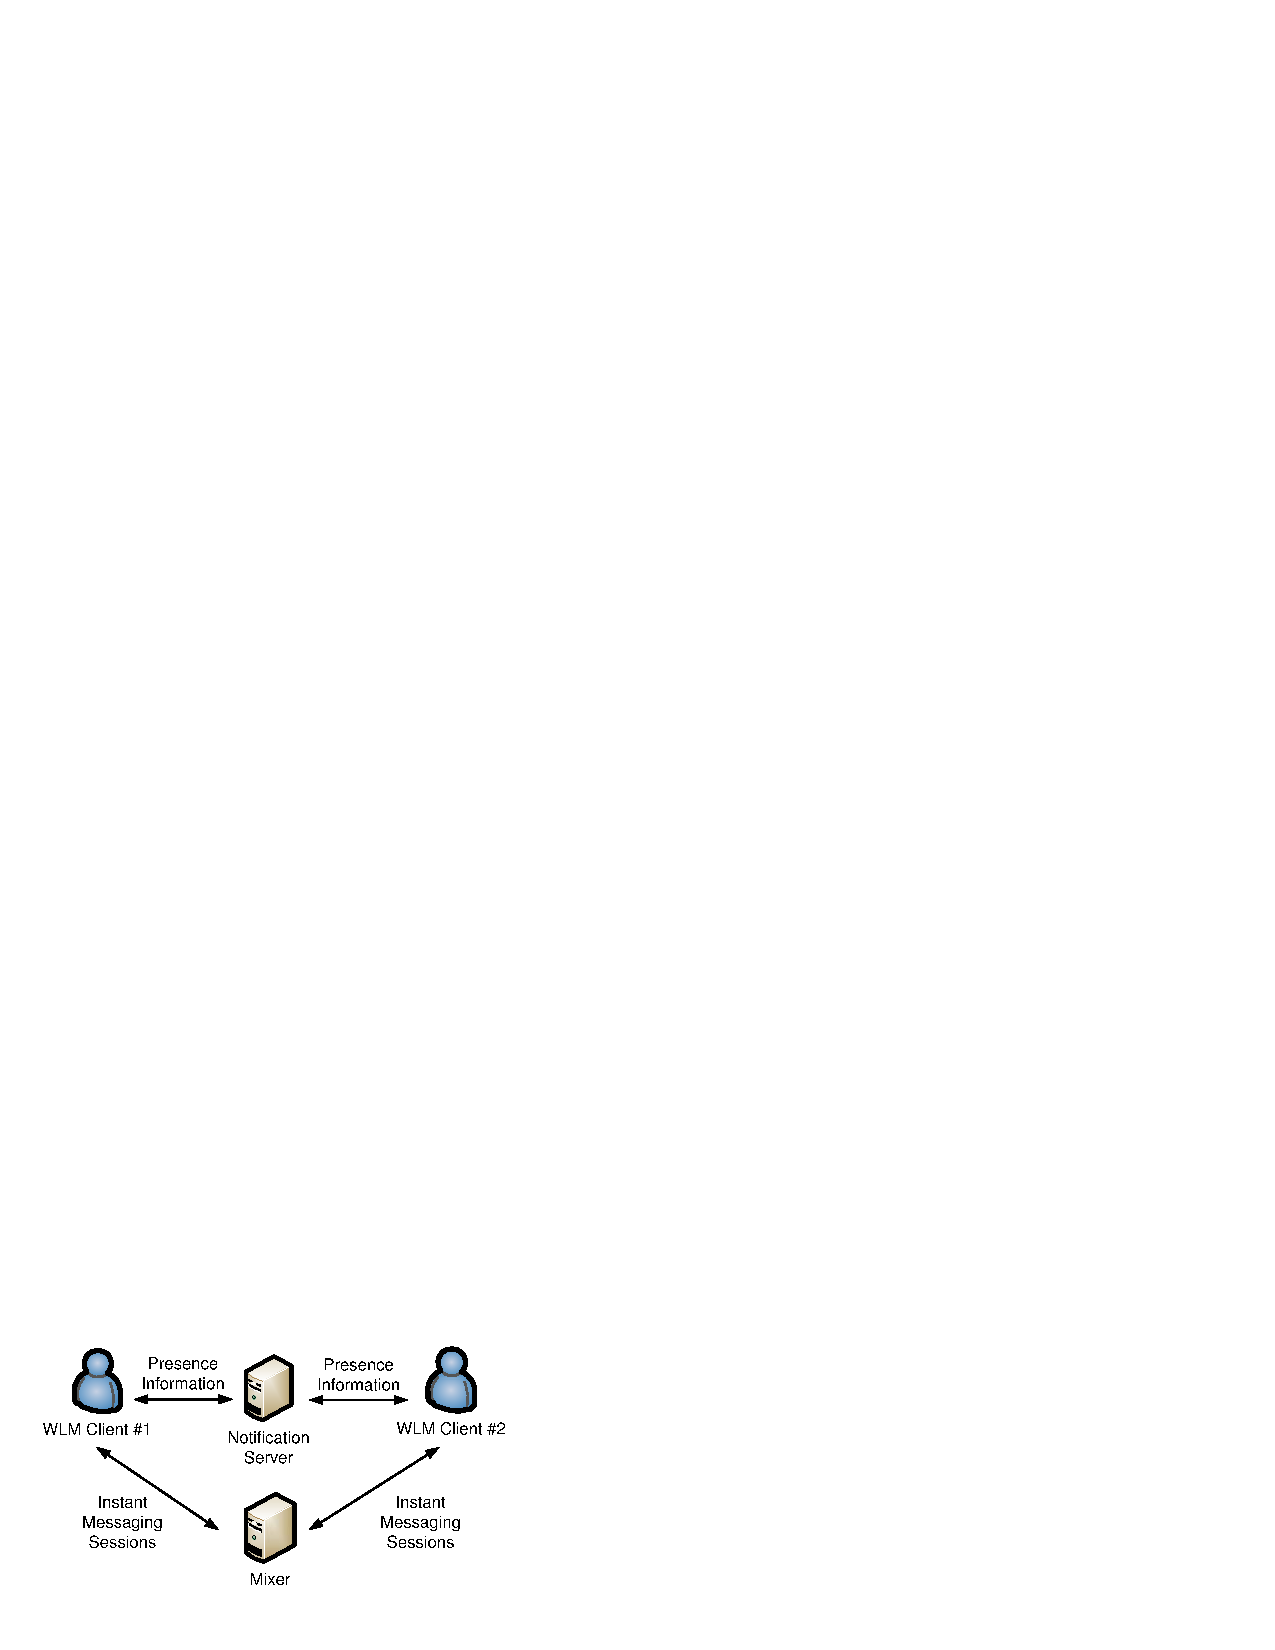
\includegraphics[width=\columnwidth]{figures/net_infrastructure}
\caption{.NET Messenger Service Infrastructure}
\label{fig:.NET Messenger Service Infrastructure}
\end{figure}

\subsection{Microsoft Notification Protocol}

MSNP is a text-based application protocol used for communication between WLM clients and the .NET Messenger Service.
Although the protocol was first intended to be an open standard \cite{fout:insidewlm}, it has since become proprietary and has undergone numerous revisions.
However, due to the unencrypted nature of the protocol, attempts to reverse-engineer the protocol have proven successful \cite{hypothetic:msnp, msnfanatic:msnp}.

The protocol consists of a series of UTF-8 and URL/XML encoded commands; each MSNP command is represented by three capital letters (e.g., command PNG represents ping).

\begin{table*}[tbh!]
\centering
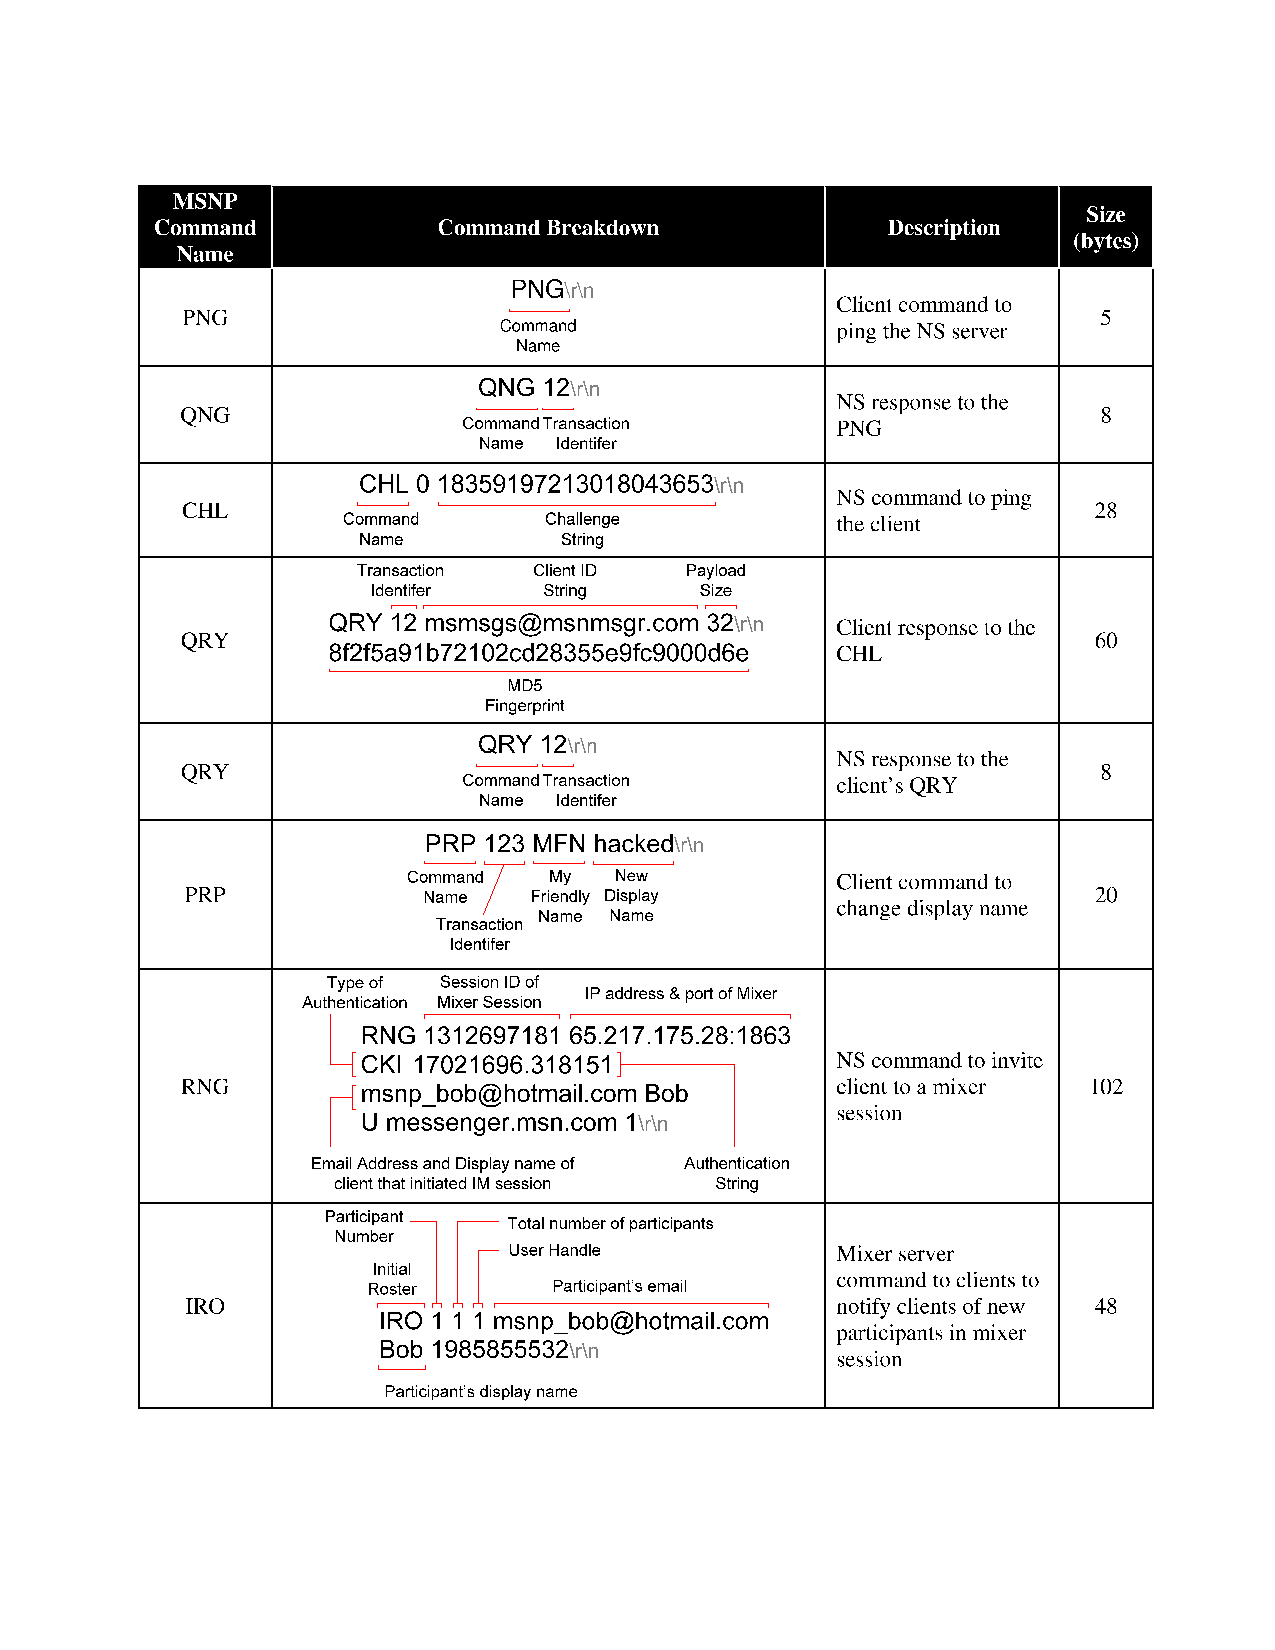
\includegraphics{figures/msnpcommands}
\caption{MSNP Commands}
\label{fig:MSNP Commands}
\end{table*}

In order to determine the validity of a persistent connection between the NS and the client, MSNP allows for asynchronous bi-directional pings; both the WLM client and the NS have the ability to initiate a ping.
Pings from the client to the NS are achieved through the PNG command; the NS uses the CHL command to ping the client.
If the receiver of the ping does not respond within a predetermined time slot, disconnection from the messaging service typically follows. The time slot varies between the various IM applications. For example, in WLM, the official MSNP IM application, the client pings the NS approximately every 45 seconds whereas in alternative IM applications such as Pidgin \cite{pidgin:url}, the pings occur approximately every minute.
Note that the ping-response initiated by the NS entails three transactions (CHL-QRY-QRY).
Table 1 specifies the structure of those MSNP commands that are relevant to our ABTH-based attack on the WLM.

Within this timeframe, ABTH can exploit these two sets of ping-response commands to eliminate the discrepancy between the sequence and ack numbers of the client and the NS TCP stacks created by the injection of a TCP packet. In doing so, an attacker has the capability of injecting any number of spoofed MSNP commands without disconnecting the underlying TCP session.
Although some MSNP commands require a pseudo-random number or hash value (e.g., challenge string, MD5 fingerprint), these values do not have to be correct for the purpose of mounting an ABTH attack. Furthermore, MSNP commands are terminated by carriage return ($\backslash$r$\backslash$n or 0x0d0a), which has a size of 2 bytes.
Due to the MSNP specification�s flexibility with white-space padding, additional white space can be added to the packet following the carriage return. By artificially inflating the packet size, the ABTH calculations are greatly simplified and the number of packets necessary to re-synchronize the TCP connection can be reduced.

In order to demonstrate the feasibility of ABTH, the follow sections will demonstrate the spoofing of MSNP commands without causing the disconnection of the MSNP connection. Two spoofing attacks will be described: display name spoofing and identity spoofing. Both attacks use the official WLM client as well as the live .NET Messaging Service. In the identity spoofing attack, a rogue WLM mixer server was implemented where the official Microsoft WLM client will connect to.

\subsection{Display Name Spoofing}

By injecting the MSNP command, PRP, an attacker is capable of modifying a victim's display name to an arbitrary string. The structure of PRP is shown in Table 1.

The NS acknowledges the PRP command by responding to the client by sending the received PRP command minus any additional white space that was added in the original PRP.
The NS will then update the user�s information resulting in presence updates pushed to all of the user's contacts.
Although all of the user's contacts are notified of the change to the victim's display name, the victim is completely oblivious to the situation and the client will not notice a change to their display name.

Following the injection of the packet, the TCP stacks of the WLM client and the NS can be resynchronized through ABTH.
For demonstration purposes, the sequence numbers of the client and the NS are assumed to be 100 and 500 prior to the spoofed packet.
During normal operation, NS ack number should match client sequence number and client ack number should match NS sequence number, as seen in the first row of Table 2.

\begin{table*}[tbh!]
\centering
{\small
\begin{tabular}{|l l l l l l l l|}
\hline
\textbf{Command}&\textbf{Direction}&\textbf{From/To}&\textbf{Data Size}&\textbf{Client Seq}&
\textbf{Client Ack}&\textbf{NS Seq}&\textbf{NS Ack}\\
\hline
	\textit{Before Attack:} & & & & 100 & 500 & 500 & 100 \\
	PRP & Sent to attacker & NS & 24 & 100 & 500 & 500 & \textbf{124} \\
	PRP & Received by attacker & NS & 20 & 100 & 500 & \textbf{520} & 124 \\
	\multicolumn{8}{|l|}{\textit{Begin ABTH:}} \\
	PNG & Sent to attacker & NS & 6 & 100 & 500 & 520 & \textbf{130} \\
	QNG & Received by attacker & NS & 8 & 100 & 500 & \textbf{528} & 130 \\
	\multicolumn{8}{|l|}{\textit{Repeat PNG/QNG exchange for 5 more times..}} \\
	CHL & Sent to attacker & Client & 60 & 100 & \textbf{560} & \textbf{568} & \textbf{160} \\
	QRY & Received by attacker & Client & 60 & \textbf{160} & 560 & 568 & 160 \\
	QRY & Sent to attacker & Client & 8 & 160 & \textbf{568} & 568 & 160 \\
\hline
\end{tabular}}
\caption{Display Name Spoofing}
\label{tb:dispNameSpoofing}
\end{table*}

While the sequence numbers of the NS or the client cannot be controlled, the ack numbers of both sides can be altered by spoofing a whitespace-padded packet.
Table 3 shows the amount of padding that used for this example.
Each command is sent or received by the attacker in the order listed in Table 2.

As the last row of Table 2 shows, with the client's sequence number equal to the NS's ack number, and the NS's sequence number equal to the client's ack number, ABTH has successfully completed its series of application specific commands, and the TCP connection is returned to a synchronized state and is ready to transmit further legitimate and/or illegitimate packets.

\begin{table*}[tbh!]
{\small
\hfill{}
\begin{tabular}{|l l l l|}
\hline
&\textbf{Command}&\textbf{Size Before Padding}&\textbf{Size After Padding}\\
\hline
	Name change & PRP 123 MFN hacked$\backslash$r$\backslash$n & 20 & 24 \\
	Client ping & PNG$\backslash$r$\backslash$n & 5 & 6 \\
	Server ping & CHL 0 8359197213018043653$\backslash$r$\backslash$n & 28 & 60 \\
	Server ping response & QRY 12$\backslash$r$\backslash$n & 8 & 8 \\
\hline
\end{tabular}}
\hfill{}
\caption{Display Name Spoofing Padded Commands}
\label{tb:dispNameSpoofingCmds}
\end{table*}

\subsection{Identity Spoofing}

By exploiting the same vulnerability, ABTH can be used to spoof the identities of WLM users.
As illustrated in Figure 2, when a user wishes to initiate a conversation with another contact, the user first requests an IM session through the NS.
The NS returns a session authentication ID and network destination IP address and port that points to a mixer.
The client then establishes a persistent TCP connection to the designated mixer.
Once the client�s connection to the mixer has been established, the client proceeds to invite other contacts to join the conversation.
Each invited contact receives an invite through their NS connection to connect to the specified mixer.
Once all parties are connected to the mixer, the mixer relays all instant messages to the WLM clients.

% Insert IM Initiation sequencing diagram here

In order to spoof an instant messaging session, a spoofed invite message is injected to the victim (step 4 of Figure 2).
As shown in Table 1, the invite message contains the address of a mixer server of our designation and the identity of the contact that we wished to impersonate, in this case Bob.

Upon receiving the invite message, Alice will establish a connection to the address of the mixer server specified in the invite message, which in this scenario will be rogue mixer server. As a result of the injected invite, the TCP connection between the NS and Alice's WLM client are now out of sync.
Thus, ABTH is employed to mask the effects of the injected packets.

\begin{center}
\begin{table*}[tbh!]
{\small
\hfill{}
\begin{tabular}{|l p{5cm} l l|}
\hline
&\textbf{Command}&\textbf{Size Before Padding}&\textbf{Size After Padding}\\
\hline
	Mixer invite & RNG 1312697181 65.217.175.28:1863 CKI 17021696.318151 msnp\_bob@hotmail.com Bob U messenger.msn.com 1$\backslash$r$\backslash$n & 102 & 120 \\
	Client ping & PNG$\backslash$r$\backslash$n & 5 & 5 \\
	Server ping & CHL 0 8359197213018043653$\backslash$r$\backslash$n & 28 & 28 \\
	Server ping response & QRY 12$\backslash$r$\backslash$n & 8 & 8 \\
\hline
\end{tabular}}
\hfill{}
\caption{Identity Spoofing Padded Commands}
\label{tb:identitySpoofingCmds}
\end{table*}
\end{center}

% Insert packet exchange of identity spoofing table here

Once connected to the victim, the rogue mixer server will send the identities of the participants already in the messaging session through the IRO command, which in this case is Bob only, as shown in Table 1.
At this point, the rogue mixer server has established a legitimate TCP connection with the victim and no additional attack packets are required to send messages to Alice on behalf of Bob.

Alice's WLM client will recognize the Bob�s email and display name as a contact on their contact list, and the client will assume that an authentic instant messaging session had been established with Bob (msnp\_bob@hotmail.com).
Through the rogue mixer server, an attacker is able to impersonate Bob and can send any number of instant messages to Alice with Alice unable to determine the distinction between the attacker and the real Bob.

\section{Discussion}

Our experiments demonstrate that MSNP can be successfully attacked by through ABTH. However, ABTH has several caveats.

\subsection{Limitations}

In the case with WLM, it is crucial that ABTH is completed prior to the next client ping, which occurs in roughly 45 seconds.
Otherwise, the client would repeatedly ping the NS and discover the imbalance in sequence numbers evntually leading to a timeout and disconnection.
Depending on the resources of the attacker, ABTH can be reasonably accomplished within this timeframe, as our experiments demonstrated.

ABTH requires the length of responses be greater than the commands issued to provoke them.
If this was not the case, resynchronization would only widen the gap of mismatched seqnums.
Similarly, application commands with similar behaviour to NOP (no operation) that do not require responses would not work either.

Our implementation of ABTH on the MSNP protocol calculates and generates the required commands to send prior to the attack and are therefore static.
If either host sends packets during the restoration phase, this would result in ABTH to fail in resynchronizing their TCP stacks.
As a result, no network traffic can occur while ABTH is in the process of sending its own packets.
Complex algorithms capable of adjusting to live traffic dynamically may improve this performance.

\subsection{Countermeasures}

A straight-forward countermeasure against ABTH is to encrypt all application traffic with SSL/TLS to authenticate messages.
However, large-scale applications such as IM applications that use MSNP would require substantial server resources in encrypting all network traffic.

Some applications may connect peers to peers, as MSNP does implicitly by allowing a communication channel between two clients.
In such cases, clients may encrypt traffic and authenticate each other through the channel provided by the application.
As a case in point, SimpLite-MSN \cite{secway:url} sets up RSA keys and authenticates all instant messaging traffic for MSNP, providing protection against spoofing.

Intrusion detection systems (IDS) may possibily detect ABTH given a well characterized behaviour of attacks.
Since ABTH utilizes minimal resources and is limited to the specification of TCP and the application, the behaviour would need to be described precisely, which may or may not be feasible as it may step within boundaries of legitimate application traffic.

Even if packets are sent in plain text, a simple regulatory mechanism of the application protocol could present some integrity with each message, such as tagging application messages with sequence numbers.
It would be difficult to inject a packet and expect further messages to be accepted since the application also keeps track of the list of messages.
This straightforward yet non-trivial detail also alleviates the application protocol from its dependence on the network layer and the assumption that packets on the network layer are authentic.

For network service providers, the most effective method to disable ABTH and message spoofing all together would be to restrict IP packets containing designated source IP addresses for each port of a switched network \cite{templeton:spoof}.
However, this method would be ineffective in a wireless medium, such as WiFi.
Of course, encryping of WiFi traffic would circumvent ABTH.

\subsection{Feasibility}

Our particular implementation of ABTH on MSNP completes within roughly 2 seconds and is triggered on the receiving of a MSNP PNG command.
Although the amount of MSNP traffic varies depending on the time of day, number of contacts, and other factors, the logs obtained through monitoring several days of network traffic have concluded that probability of network traffic occurring within 2 seconds of a ping is less than 5\%.
As such, ABTH would prevail over 95\% of the time, a large concern for potential threat.

In environments that provide a common physical communication medium, ABTH may present a threat.
Examples include hubbed networks, coffee shops that offer WiFi service, and increasingly popular virtualized servers.
Application protocols vulnerable to ABTH, such as MSNP, were not designed to offer secure communication channels.
It is imperative that, as protocols become more widely adopted, they are improved upon and revised to accommodate their broadening uses.

\section{Conclusion}

By combining the innocuous features of the transport and application layers and the lack of cryptographic protection at either layer, Application-Based TCP Hijacking (ABTH) offers an elegant way of exploiting certain application protocols.
Sending commands to both hosts to provoke responses allows an attacker to create a gap of a certain size in TCP sequence numbers to inject a malicious command.
We presented a proof of ABTH concept by successfully experimenting with two forms of attacks on Windows Live Messenger, Microsoft's popular instant messaging application, which runs over the Microsoft Notification Protocol (MSNP).

While some protocols, such as MSNP, were designed to suit flexible environments, as the environment evolved, these features have become subtle vulnerabilities.
Although hardware Ethernet equipment has been updated to obstruct lower level attacks (e.g., ARP poisoning), the realm of attacks is reaching beyond the protection capabilities of network devices.

\bibliographystyle{abbrv}
\bibliography{abthmsnp}

\end{document}
